\documentclass{beamer}
% Required packages
\usepackage{amsmath}
\usepackage{physics}
\usepackage{graphicx}
\usepackage{siunitx}
\usepackage{xcolor}
% Define custom colors for DS9 theme
\definecolor{ds9blue}{RGB}{25,25,112}
\definecolor{ds9gold}{RGB}{218,165,32}
\definecolor{ds9grey}{RGB}{105,105,105}
\definecolor{ds9red}{RGB}{178,34,34}
% Set up the Madrid theme with custom colors
\usetheme{Madrid}
\usecolortheme{whale}
\setbeamercolor{palette primary}{bg=ds9blue,fg=white}
\setbeamercolor{palette secondary}{bg=ds9grey,fg=white}
\setbeamercolor{palette tertiary}{bg=ds9gold,fg=black}
\setbeamercolor{palette quaternary}{bg=ds9red,fg=white}
\setbeamercolor{structure}{fg=ds9blue}
\setbeamercolor{title}{fg=ds9gold}
\setbeamercolor{subtitle}{fg=ds9gold}
\setbeamercolor{frametitle}{bg=ds9blue,fg=white}
\setbeamercolor{block title}{bg=ds9blue,fg=white}
\setbeamercolor{block body}{bg=ds9grey!20,fg=black}

\title[NOPS Exam Guide]{Scannable Exam Guide}
\subtitle{How to Successfully Complete Your NOPS Answer Sheet}
\author[Mr. Gullo]{Mr. Gullo}
\date[June 2025]{June, 2025}

\begin{document}

\frame{\titlepage}

\section{Introduction to NOPS Exams}

\begin{frame}{Learning Objectives}
\frametitle{Learning Objectives}
By the end of this presentation, you will be able to:
\begin{itemize}
\item Properly handle and maintain your NOPS answer sheet
\item Correctly fill out your personal information and registration number
\item Mark multiple-choice answers using the proper technique
\item Follow correct procedures for written responses
\item Apply appropriate error correction protocols
\item Complete a final checklist before submission
\end{itemize}
\end{frame}

\begin{frame}{What is a NOPS Exam?}
\frametitle{What is a NOPS Exam?}
\begin{block}{NOPS Definition}
NOPS stands for \textbf{Network Optical Processing System} - a computer-based grading system that scans your answer sheet optically.
\end{block}

\textbf{Key Features:}
\begin{itemize}
\item Computer scanner reads your markings
\item Extremely sensitive to marks and placement
\item Requires precise technique for accurate grading
\item Any errors in marking can result in incorrect scoring
\end{itemize}

\end{frame}

\section{Answer Sheet Procedures}

\begin{frame}{Answer Sheet Handling}
\frametitle{Answer Sheet Handling}
\begin{block}{Critical Rule}
The scanner is \textbf{very sensitive} - treat your answer sheet with extreme care!
\end{block}

\textbf{DO:}
\begin{itemize}
\item Keep the sheet clean, dry, and flat
\item Handle with clean hands
\item Place on a flat, stable surface when marking
\end{itemize}

\textbf{DO NOT:}
\begin{itemize}
\item Fold, crease, or tear the sheet
\item Spill liquids or get the sheet wet
\item Write notes or doodles outside designated areas
\item Rest your hand heavily on the sheet while marking
\end{itemize}
\end{frame}

\section{Filling Information}

\begin{frame}{Required Materials}
\frametitle{Required Materials}
\begin{block}{Pen Requirement}
Use \textbf{ONLY} a blue or black pen as instructed on the answer sheet.
\end{block}

\textbf{Why pen only?}
\begin{itemize}
\item Pencil marks may be too light for scanner detection
\item Erasures leave marks that confuse the scanner
\item Pen provides consistent, dark marks
\end{itemize}

\textbf{Personal Information:}
\begin{itemize}
\item Write your name clearly in the designated space
\item Add your signature where indicated
\item Use legible handwriting
\end{itemize}
\end{frame}

\begin{frame}

\begin{figure}
    \centering
    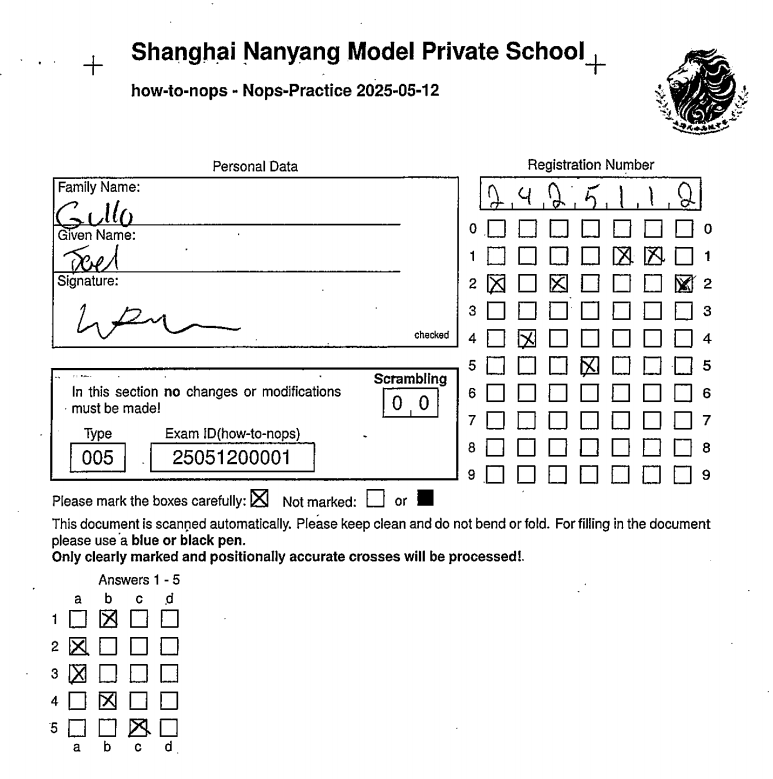
\includegraphics[width=0.5\linewidth]{scannops.png}
\end{figure}
\end{frame}

\begin{frame}{Registration Number Process}
\frametitle{Registration Number - CRITICAL STEP}
This is a \textbf{two-step process} that must be completed perfectly:

\begin{block}{Step A: Write the Digits}
Carefully write your registration number in the boxes at the top of the grid, placing \textbf{one digit per box}.
\end{block}

\begin{block}{Step B: Mark the Bubbles}
For each digit you wrote, find the matching bubble in the column directly below and mark with a clear \textbf{'X'}.
\end{block}

\textbf{Example:} If your registration number is 12345:
\begin{itemize}
\item Write "1" in first box, mark "1" bubble below
\item Write "2" in second box, mark "2" bubble below
\item Continue for all digits
\end{itemize}
\end{frame}

\begin{frame}{Pre-Filled Sections}
\frametitle{Pre-Filled Sections}
\begin{block}{Important Warning}
You will see sections labeled "Exam ID," "Type," and "Scrambling" that are already filled out.
\end{block}

\textbf{DO NOT:}
\begin{itemize}
\item Make any changes to these sections
\item Add any marks or annotations
\item Write over existing marks
\item Attempt to "correct" what appears to be errors
\end{itemize}

These sections are pre-configured for your specific exam and any changes will cause scoring errors.

\end{frame}

\section{Answering Questions}

\begin{frame}{Multiple-Choice Technique}
\frametitle{Multiple-Choice Answering}
\begin{block}{Marking Technique}
Mark your chosen answer with a clear \textbf{'X'} that fits completely inside the designated box.
\end{block}

\textbf{Step-by-step process:}
\begin{enumerate}
\item Find the question number on the answer grid
\item Locate your chosen answer (a, b, c, or d)
\item Make a clear 'X' mark inside the box
\item Ensure the 'X' does not extend outside the box boundaries
\end{enumerate}

\textbf{Critical Rule:} Mark \textbf{ONLY ONE} answer per question. Multiple marks will be scored as incorrect, even if one of them is the right answer.
\end{frame}

\begin{frame}{Written Response Guidelines}
\frametitle{Written Response Guidelines}
For questions requiring written solutions:

\begin{block}{Answer Location}
Use the separate answer page with large, numbered boxes corresponding to each open-response question.
\end{block}

\textbf{Writing Requirements:}
\begin{itemize}
\item Write your \textbf{entire answer} inside the designated box
\item Include all work, calculations, and explanations
\item Keep all writing within the box borders
\item Use clear, legible handwriting
\end{itemize}

\textbf{Important:} The scanner will \textbf{not read} anything written outside the box boundaries.

\end{frame}

\section{Error Correction}

\begin{frame}{Correcting Mistakes}
\frametitle{How to Correct a Mistake}
\begin{block}{The Problem}
Since you must use a pen, you \textbf{cannot erase} your marks.
\end{block}

\textbf{WRONG Ways to Fix Mistakes:}
\begin{itemize}
\item Crossing out the wrong answer
\item Scribbling over incorrect marks
\item Writing "wrong" next to mistakes
\item Attempting to white-out errors
\end{itemize}

\begin{block}{The ONLY Correct Solution}
Raise your hand and ask the exam supervisor for a \textbf{new answer sheet}.
\end{block}

The scanner will interpret any additional marks as errors, so a clean sheet is your only option.
\end{frame}

\section{Practice Examples}

\begin{frame}{I Do: Registration Number Example}
\frametitle{I Do: Registration Number Demonstration}
Let me show you how to properly fill out registration number \textbf{67890}:

\textbf{Step 1 - Write the digits:}
\begin{itemize}
\item Box 1: Write "6"
\item Box 2: Write "7" 
\item Box 3: Write "8"
\item Box 4: Write "9"
\item Box 5: Write "0"
\end{itemize}

\textbf{Step 2 - Mark the bubbles:}
\begin{itemize}
\item Column 1: Mark the "6" bubble with clear X
\item Column 2: Mark the "7" bubble with clear X
\item Continue for remaining digits...
\end{itemize}

\end{frame}


\section{Final Checklist}

\begin{frame}{Before You Submit}
\frametitle{Final Submission Checklist}
Complete this checklist before turning in your exam:

\begin{block}{Personal Information}
\begin{itemize}
\item[$\square$] Name written clearly
\item[$\square$] Signature provided  
\item[$\square$] Registration number digits written correctly
\item[$\square$] Registration number bubbles marked correctly
\end{itemize}
\end{block}

\begin{block}{Answer Quality}
\begin{itemize}
\item[$\square$] Every multiple-choice question has exactly one X
\item[$\square$] All marks are dark and clear
\item[$\square$] Written responses are inside designated boxes
\end{itemize}
\end{block}

\begin{block}{Physical Condition}
\begin{itemize}
\item[$\square$] Answer sheet is clean and undamaged
\end{itemize}
\end{block}
\end{frame}

\begin{frame}{Quick Reference: Dos and Don'ts}
\frametitle{Quick Reference Guide}
\begin{columns}
\begin{column}{0.5\textwidth}
\textbf{✅ DO:}
\begin{itemize}
\item Use blue or black pen
\item Mark with clear X inside boxes
\item Fill registration number perfectly
\item Keep answers in designated areas
\item Ask for new sheet if you make mistakes
\item Handle sheet carefully
\end{itemize}
\end{column}

\begin{column}{0.5\textwidth}
\textbf{❌ DON'T:}
\begin{itemize}
\item Fold, crease, or damage paper
\item Mark more than one answer per question
\item Cross out mistakes
\item Write outside answer areas
\item Use pencil or erasers
\item Modify pre-filled sections
\end{itemize}
\end{column}
\end{columns}

\begin{block}{Remember}
When in doubt, ask your exam supervisor for help!
\end{block}
\end{frame}

\begin{frame}{Summary}
\frametitle{Key Takeaways}
\textbf{Success with NOPS exams requires:}
\begin{enumerate}
\item Careful handling of your answer sheet
\item Precise completion of personal information
\item Proper marking technique for all answers
\item Following error correction protocols
\item Thorough final review before submission
\end{enumerate}

\begin{block}{Final Thought}
The computer scanner is precise but unforgiving. Your attention to detail in following these procedures will ensure your knowledge is accurately reflected in your exam score.
\end{block}

\textbf{Good luck on your exam!}

\end{frame}


\begin{frame}{Frame Title}
    $\omega$
\end{frame}

\end{document}